\documentclass[12pt]{article}

  \usepackage[polish]{babel}
  \usepackage[utf8]{inputenc}
  \usepackage[T1]{fontenc} 
  \usepackage{hyperref}
  
  \usepackage[numbers,sort&compress]{natbib}
  \usepackage{hypernat}

  \usepackage{graphicx}
  \usepackage{epstopdf}


\begin{document}
  \section{Wstęp}
  Model Fitzhugh-Nagumo, zwany dalej FHN, jest jedną z uproszczonych wersji modelu Hodgkina-Huxley'a i modeluje za pomocą dwóch równań różniczkowych zachowanie neuronu czuciowego (sensory neuron). Formalna postać modelu zaproponowanego przez R. Fitzhugha i J. Nagumo jest bardzo ogólna i łatwa do znalezienia np. na Wikipedii: \url{http://en.wikipedia.org/wiki/FitzHugh%E2%80%93Nagumo_model}.
  
  Układ tych równań w wersji analizowanej w niniejszym referacie opiera się na pracy Andre Longina i przedstawia się następująco: 

  \begin{equation} \label{eq:v}
    \epsilon \frac{dv}{dt} = v(v-a)(1-v)- \omega + \xi(t)
  \end{equation}

  \begin{equation} \label{eq:w}
    \frac{d \omega}{dt} = v - d \omega - [b + r sin(\beta t)]
  \end{equation}

  W modelu FHN \emph{v(t)} pełni rolę szybkozmiennego ''potencjału'' (odpowiednik biologicznego potencjału czynnościowego neuronu), natomiast $\omega (t)$ pełni rolę wolnozmiennej ''relaksacji''.

  Jako układ dwóch równań różniczkowych ze składnikiem stochastycznym ($\xi(t)$ - szum), model FHN spełnia kryterium układu chaotycznego (nieliniowego). Dodatkowo jest to model elementu wzbudnego: jeśli zewnętrzny bodziec (tu: składnik w nawiasie kwadratowym, czyli pobudzenie sygnałem periodycznym) przekroczy pewną wartość progową, potencjał v gwałtownie wzrośnie żeby po chwili zostać zrelaksowanym z powrotem do wartości ''spoczynkowej''.

  Ze względu na ww. zachowanie, czyli powstanie piku potencjału po przekroczeniu pewnej wartości progowej w pobudzeniu, układ był badany przez Andre Longtina pod kątem występowania rezonansu stochastycznego.

  Rezonans stochastyczny (SR) jest zjawiskiem występującym w układach sterowanych co najmniej dwoma sygnałami, z których jeden jest periodyczny, drugi natomiast jest szumem. O występowaniu rezonansu stochastycznego mówimy, kiedy nałożenie sygnału periodycznego i niezerowego szumu skutkuje wysoką periodycznością sygnału wyjściowego.
  
  Powyższe oznacza, że odpowiednio dobrany szum potrafi wzmacniać i wydobywać z układu sygnał periodyczny. Szum, zazwyczaj traktowany jako zjawisko niepożądane ze względu na obniżanie dokładności pomiaru, w układach z rezonansem stochastycznym staje się zjawiskiem jak najbardziej pożądanym.

  W swojej pracy Longtin zaobserwował zjawisko SR w (symulowanym) układzie modelowanym według przedstawionych powyżej równań. Znalazł też optymalne wartości parametrów tego równania, pozwalające na maksymalizację SNR (signal-to-noise ratio).

  Celem niniejszego referatu jest zbadanie zachowania (symulowanego) neuronu według modelu FHN wraz ze zmianą parametrów równania, jak ich zmiana wpływa na widmo fourierowskie sygnału wyjściowego (rozumianego jako pomiar potencjału w czasie).

  \section{Wyniki}
  
  Parametry do zbadania: skalowanie szumu (D), skalowanie sygnału periodycznego (r).

  Wszystkie symulacje uruchomione zostały z pobudzeniem periodycznym o okresie 1 [s] oraz krokiem iteracji dt=0.00390625 [s] (1/256 sekundy). Po 2048 iteracjach ''rozruchowych'' następowało 8192 iteracji właściwych, podczas których zapisywano wartości potencjału czynnościowego v.

  Szum skorelowany, generowany w procesie Ornsteina-Uhlenbecka, mnożony jest przez $\sqrt{2D}$.


  \subsection{Skalowanie szumu (D)}

  Longtin w swojej pracy podał optymalną wartość D ($10^{-5}$), powodującą (wraz z innymi parametrami). W niniejszym eksperymencie wartość r wynosiła 0.08, tyle ile podczas większości symulacji wykonanych w ramach zbierania danych do mojej pracy dyplomowej. Zmiany w widmie mocy wraz ze zmianą D są przedstawione na wykresach.

  \begin{figure}
  \centering
  \begin{tabular}{cc}
    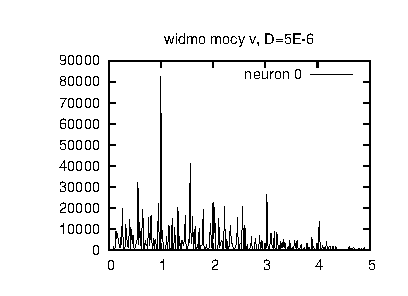
\includegraphics{referat_graph/D5e-6.eps} & 
    \includegraphics{referat_graph/D8e-6.eps} \\
    \includegraphics{referat_graph/D1e-5.eps} &
    \includegraphics{referat_graph/D1e-5_2.eps} \\
    \includegraphics{referat_graph/D2e-5_2.eps} &
    \includegraphics{referat_graph/D4e-5.eps} \\
    \includegraphics{referat_graph/D8e-5_2.eps} &
    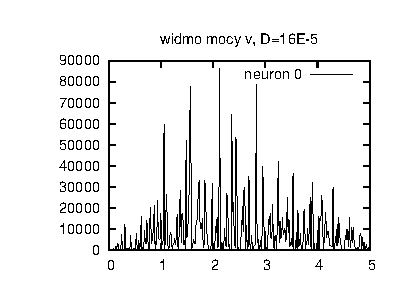
\includegraphics{referat_graph/D16e-5.eps} 
  \end{tabular}
  \end{figure}


  \subsection{Skalowanie sygnału periodycznego (r)}

  Longtin w swojej pracy badał zachowanie modelu FHN dla różnych wartości r, w zakresach 0.05-0.4. W swojej pracy dyplomowej oraz niniejszym eksperymencie symulacje uruchamiałem z optymalną wartością D ($10^{-5}$). Zmiany w widmie mocy wraz ze zmianą D są przedstawione na wykresach.

  \begin{figure}
  \centering
  \begin{tabular}{cc}
    \includegraphics{referat_graph/r001.eps} &
    \includegraphics{referat_graph/r003.eps} \\
    \includegraphics{referat_graph/r005.eps} & 
    \includegraphics{referat_graph/r010.eps} \\
    \includegraphics{referat_graph/r020_2.eps} &
    \includegraphics{referat_graph/r040_2.eps} \\
  \end{tabular}
  \end{figure}

  \section{Podsumowanie}

  Wartości parametrów wybrane przez Longtina są kompromisem pomiędzy obserwowalnym rezonansem stochastycznym (wzmocnieniem częstotliwości pobudzenia) a rezonatorem w którym szum odgrywa zbyt dużą bądź zbyt małą rolę.
  
  Badanie szerokości piku dla częstotliwości bazowej ma, w świetle przedstawionych wyżej wyników, niewiele sensu: ''rozmycie'' widma objawia nie objawia się rozszerzeniem piku głównego, lecz pojawieniem się wielu konkurencyjnych, podobnie wąskich.
  
\end{document}
